% ==========================================================================
%  Figure: Elapsed Time by K — Line Chart
% ==========================================================================
%  Required: \usepackage{pgfplots}  \pgfplotsset{compat=1.18}
% ==========================================================================

\begin{figure}[t]
\centering
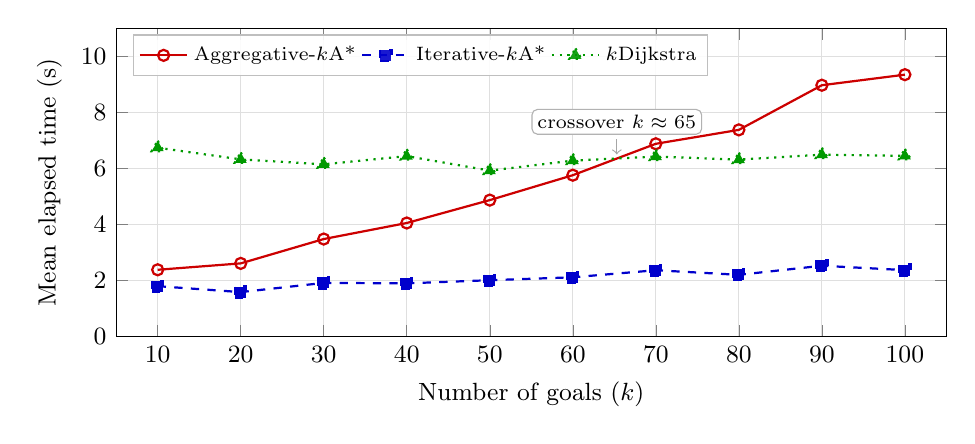
\begin{tikzpicture}
\begin{axis}[
    width=\columnwidth,
    height=5.5cm,
    xlabel={Number of goals ($k$)},
    ylabel={Mean elapsed time (s)},
    xmin=5, xmax=105,
    ymin=0, ymax=11,
    xtick={10,20,30,40,50,60,70,80,90,100},
    ytick={0,2,4,6,8,10},
    grid=major,
    grid style={gray!25},
    tick label style={font=\small},
    label style={font=\small},
    legend style={
        at={(0.02,0.98)},
        anchor=north west,
        font=\scriptsize,
        draw=gray!50,
        fill=white,
        fill opacity=0.9,
        text opacity=1,
        row sep=-1pt,
        inner sep=2pt,
        legend columns=3,
    },
    legend cell align={left},
    cycle list name=color list,
]

% Aggregative-kA*
\addplot[
    color=red!80!black,
    mark=o,
    mark size=2pt,
    thick,
    solid,
] coordinates {
    (10,2.388) (20,2.616) (30,3.484) (40,4.056) (50,4.872)
    (60,5.76) (70,6.88) (80,7.376) (90,8.968) (100,9.344)
};
\addlegendentry{Aggregative-$k$A*}

% Iterative-kA*
\addplot[
    color=blue!80!black,
    mark=square*,
    mark size=2pt,
    thick,
    dashed,
] coordinates {
    (10,1.804) (20,1.592) (30,1.92) (40,1.904) (50,2.016)
    (60,2.12) (70,2.372) (80,2.208) (90,2.532) (100,2.376)
};
\addlegendentry{Iterative-$k$A*}

% kDijkstra
\addplot[
    color=green!60!black,
    mark=triangle*,
    mark size=2.5pt,
    thick,
    dotted,
] coordinates {
    (10,6.74) (20,6.324) (30,6.148) (40,6.44) (50,5.924)
    (60,6.28) (70,6.424) (80,6.316) (90,6.492) (100,6.448)
};
\addlegendentry{$k$Dijkstra}

% Crossover annotation
\node[
    fill=white,
    draw=gray!60,
    rounded corners=2pt,
    inner sep=2pt,
    font=\scriptsize,
    anchor=south,
] at (axis cs:65.3,7.2) {crossover $k \approx 65$};
\draw[->, gray!70, thin] (axis cs:65.3,7.05) -- (axis cs:65.3,6.5);

\end{axis}
\end{tikzpicture}
\caption{Mean elapsed time as a function of goal count~$k$, averaged
over all 2{,}500 problem instances (250 per $k$-value). Distinct
markers and line styles distinguish the three algorithms. The vertical
arrow marks the crossover point ($k \approx 65$) where
Aggregative-$k$A* becomes slower than $k$Dijkstra.}
\label{fig:elapsed_by_k}
\end{figure}
